\section{Autoencoders}

\subsection{Nota su PCA}

La PCA (Principal Component Analysis) è una tecnica di riduzione della
dimensionalità che si basa sulla decomposizione in autovalori della matrice di
covarianza.

Ora, immaginiamo di avere tre input $x_1, x_2, x_3$. Un \textbf{neurone} può
essere visto come una combinazione lineare di questi tre input, ovvero:

\begin{equation}
    y = w_1x_1 + w_2x_2 + w_3x_3
\end{equation}

\subsection{Autoencoders}

E' un architettura che permette di \textbf{proiettare} il nostro input in uno
\textbf{spazio dimensionale più piccolo}.

Avendo un input $x_1, x_2, x_3$, la rete ci darà come \textit{output} la
\textbf{ricostruzione} dell'input.

\begin{quote}
    Obiettivo: minimizzare la differenza tra l'input e la sua ricostruzione
\end{quote}

%Grafico di una rete con input x1,x2,x3. primo layer nascosto 3 nodi, secondo layer 2 nodi, terzo layer 3 nodi, output x1',x2',x3'

\begin{figure}[H]
    \begin{center}
        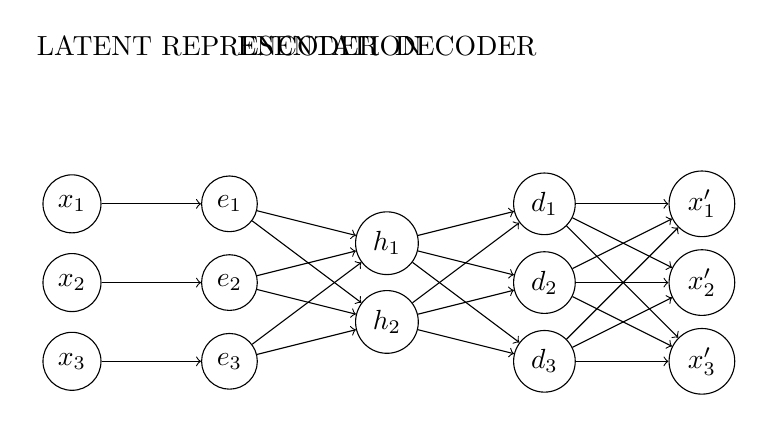
\begin{tikzpicture}
            \node[draw, circle] (x1) at (0, 0) {$x_1$};
            \node[draw, circle] (x2) at (0, -1) {$x_2$};
            \node[draw, circle] (x3) at (0, -2) {$x_3$};
            \node[draw, circle] (e1) at (2, 0) {$e_1$};
            \node[draw, circle] (e2) at (2, -1) {$e_2$};
            \node[draw, circle] (e3) at (2, -2) {$e_3$};

            %draw 2 nodes between the output and the hidden layer

            \node[draw, circle] (h1) at (4, -0.5) {$h_1$};
            \node[draw, circle] (h2) at (4, -1.5) {$h_2$};

            \node[draw, circle] (d1) at (6, 0) {$d_1$};
            \node[draw, circle] (d2) at (6, -1) {$d_2$};
            \node[draw, circle] (d3) at (6, -2) {$d_3$};

            \node[draw, circle] (xp1) at (8, 0) {$x'_1$};
            \node[draw, circle] (xp2) at (8, -1) {$x'_2$};
            \node[draw, circle] (xp3) at (8, -2) {$x'_3$};

            %write over D_1, D_2, D_3 the text ENCODER
            \node[draw=none] (t1) at (3, 2) {ENCODER};
            \node[draw=none] (t1) at (5, 2) {DECODER};
            \node[draw=none] (t1) at (2, 2) {LATENT REPRESENTATION};

            \draw[->] (x1) -- (e1);
            \draw[->] (x2) -- (e2);
            \draw[->] (x3) -- (e3);

            \draw[->] (e1) -- (h1);
            \draw[->] (e2) -- (h1);
            \draw[->] (e3) -- (h1);

            \draw[->] (e1) -- (h2);
            \draw[->] (e2) -- (h2);
            \draw[->] (e3) -- (h2);

            \draw[->] (h1) -- (d1);
            \draw[->] (h1) -- (d2);
            \draw[->] (h1) -- (d3);

            \draw[->] (h2) -- (d1);
            \draw[->] (h2) -- (d2);
            \draw[->] (h2) -- (d3);

            \draw[->] (d1) -- (xp1);
            \draw[->] (d2) -- (xp1);
            \draw[->] (d3) -- (xp1);

            \draw[->] (d1) -- (xp2);
            \draw[->] (d2) -- (xp2);
            \draw[->] (d3) -- (xp2);

            \draw[->] (d1) -- (xp3);
            \draw[->] (d2) -- (xp3);
            \draw[->] (d3) -- (xp3);

        \end{tikzpicture}
    \end{center}
\end{figure}
\begin{equation}
    Loss(\bar{x}, \bar{x'})
\end{equation}

L'\textbf{autoencoder} è praticamente l'unione tra \textbf{encoder, latent
    representation e decoder}.

\begin{domanda}(Per quale motivo usiamo le NN e non le PCA?)
\end{domanda}

La risposta è che le \textbf{PCA} sono lineari, e quindi meno complesse. Per
questo motivo, le NN sono più flessibili e possono essere usate per risolvere
problemi più complessi.

\subsubsection{Gli steps}

\begin{enumerate}
    \item Encoder: Impara una \textbf{rappresentazione compatta} dell'input
    \item Decoder: Ricostruisce l'input
\end{enumerate}

\subsubsection{Applicazioni}

Gli autoencoders possono essere usati in vari campi.

Ad esempio, forzare $x = r$. Questo porta ad un \textbf{rischio di overfitting
    elevato}. Diminuisce la dimensione e apprendimenti delle feature.

La vera potenza però è nell'\textbf{astrarre i dati} invece di impararli in
modo perfetto. Stiamo parlando di \textbf{produrre dati} che potrebbero
appartenere al dominio di input. Questo rientra in \textbf{data generation, data completion}.

Gli autoencoders non sono perfetti e soffrono di alcuni problemi. Alcuni sono:
\begin{itemize}
    \item Overfitting
    \item Grandezza del codice
\end{itemize}

Se vuoi copiarti le slides e aggiungere qualcosa.

\subsection{Autoencoders e Convolution}

Ricordiamo il concetto di fare sampling nello spazio latente. Questo è
fondamentale per la generazione di nuovi dati.

\begin{figure}[H]
    \begin{center}
        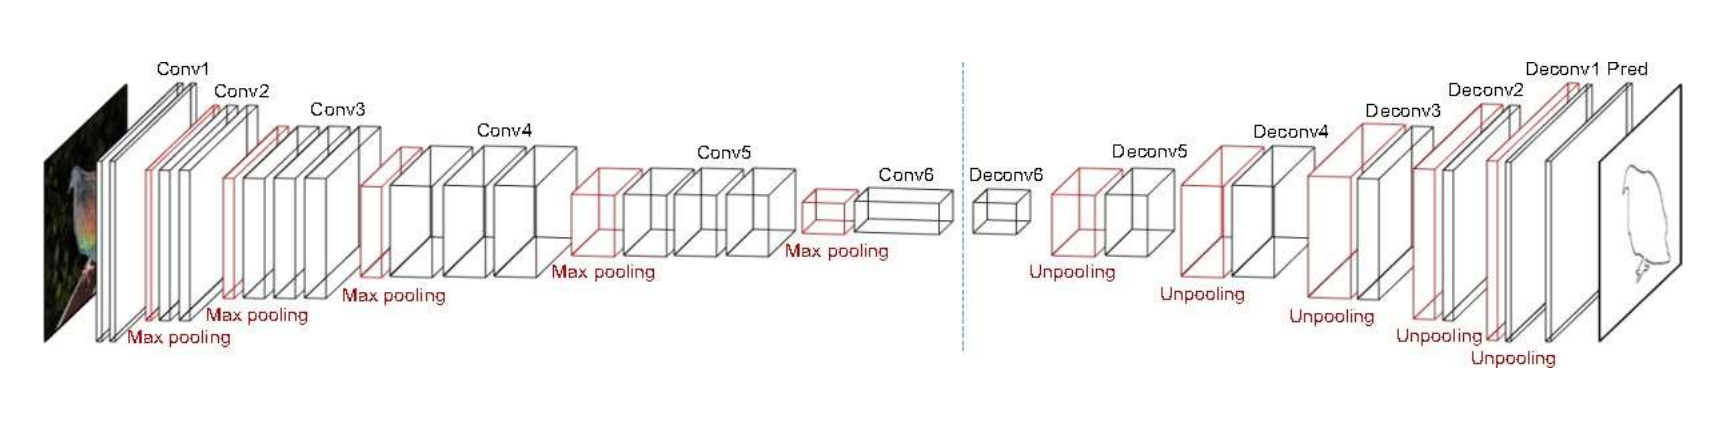
\includegraphics[scale=0.3]{images/autoencoders.png}
        \caption{Convolutional Autoencoder}
    \end{center}
\end{figure}

\begin{figure}[H]
    \begin{center}
        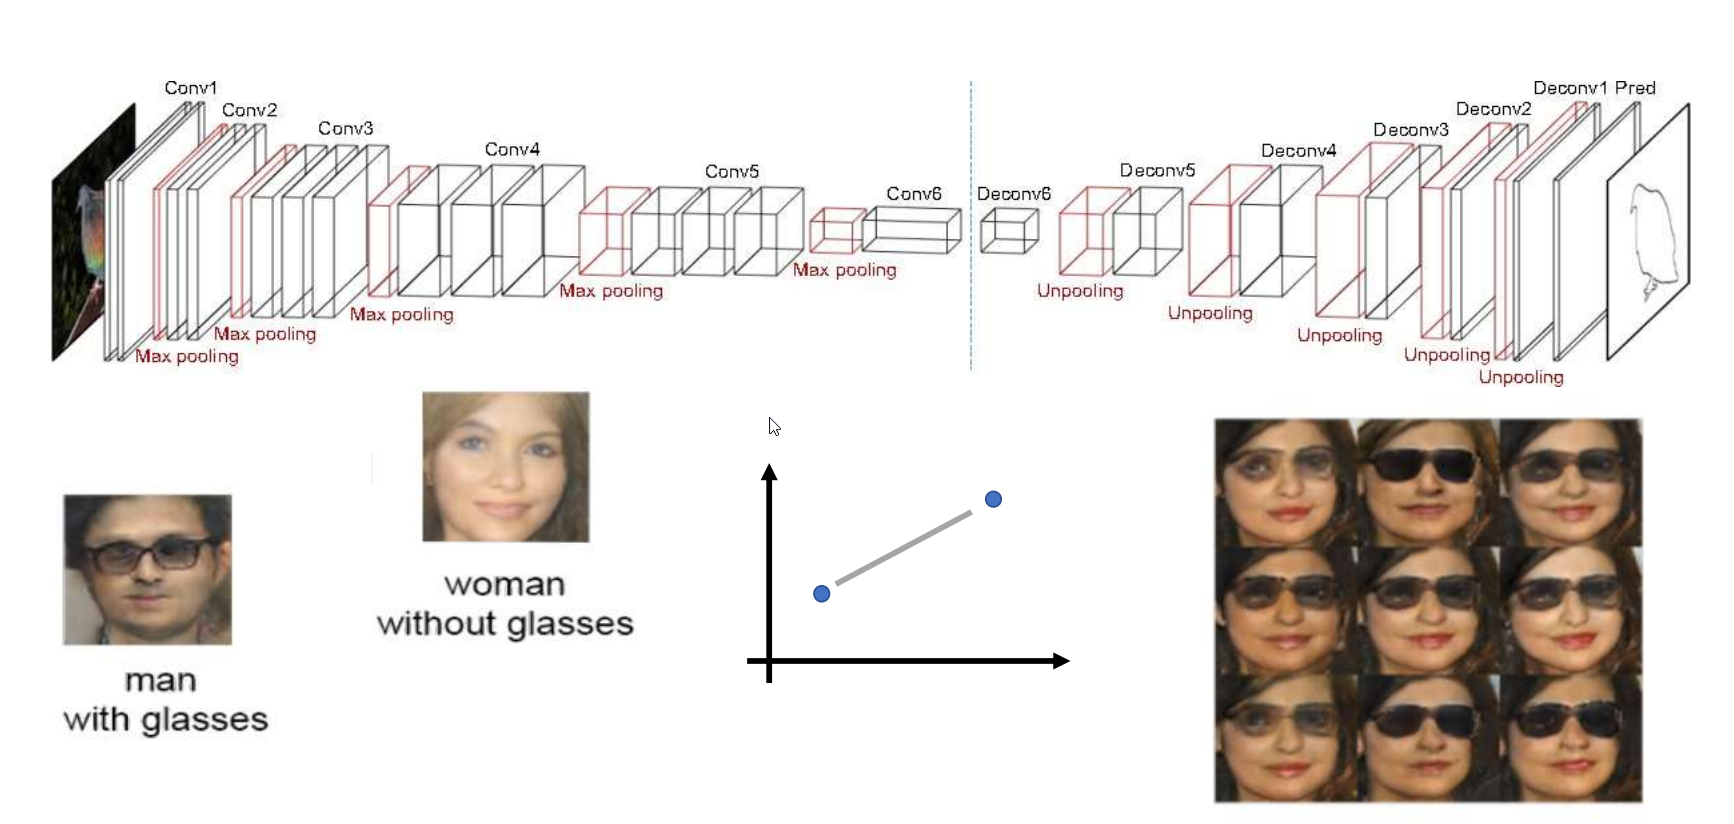
\includegraphics[scale=0.3]{images/autoencoders2.png}
        \caption{Convolutional Autoencoder sampling}
    \end{center}
\end{figure}

Praticamente, questa tecnologia è alla base per i \textbf{Deep Fakes!}

Altre informazioni: Notebook su autoencoders.
\newpage